\section{Views}
In this section, we present three prototypical views built upon the
presented visualization infrastructure. The interaction of the views provide a
scalable top-down approach for identifying hotspots, developing parallelization
strategies, and validating these strategies with respect to data dependencies.

\subsection{Performance View}
\label{sec:performance_view}
The performance view is an interactive representation of a program's profiling
and trace data (see Figure \ref{fig:emsim}). Its primary purpose is to assist
users in identifying scenarios that may benefit from parallelization. A
holistic visualization of a program's runtime behavior helps users to spot
potential performance and guides optimization efforts.

There are two visualization modes in the performance view: tracing and
profiling. The tracing mode represents an icicle plot augmented with loop
information, i.e., a hierarchical view of calls made during program execution.
The calls are arranged chronologically from left to right, and the visibility
of loop information can be toggled (on or off). Trace visualization is useful
for detailed examination of a program, especially when the invocation order is
important. The profiling mode presents the user a hierarchical view of the
functions called during execution. The length of each function in the view is
given by the sum of the calls' execution time, which is often sufficient to
quickly pinpoint hot spots.

As a program's size and complexity increases, so does the quantity of its
performance data, making the data harder to digest at once. For this reason,
the performance view provides zooming at call level and execution time
filtering. The latter sets the minimum execution time required for a call to be
loaded. The minimum value depends on the percentage of the execution time of
the current top-level call in the view. This only allows the rendering of calls
coarse enough to be easily visible. With the call zooming feature, users can
focus on a specific call, which makes it the top-level call, recomputes a new
minimum value, and loads child calls of the focused call that weren't displayed
before.

\subsection{Calling Context Tree (CCT) View}
The CCT view targets comprehension of the dynamic behavior of an application.
It displays a calling context tree consisting of call nodes, loop nodes, and
memory nodes (see Figure \ref{fig:cct_view}). Nodes for calls (or groups of
calls), loop executions, and loop iterations are positioned using a tidy tree
layout~\cite{TidierTree}. Children of nodes are vertically sorted by their
start time to reflect their execution time. Memory nodes accessed by
arbitrary tree nodes can not be integrated in a tree layout. Therefore,
they are positioned using an unconstrained layout based on a force simulation
around the rest of the tree.

\begin{figure}[h!]
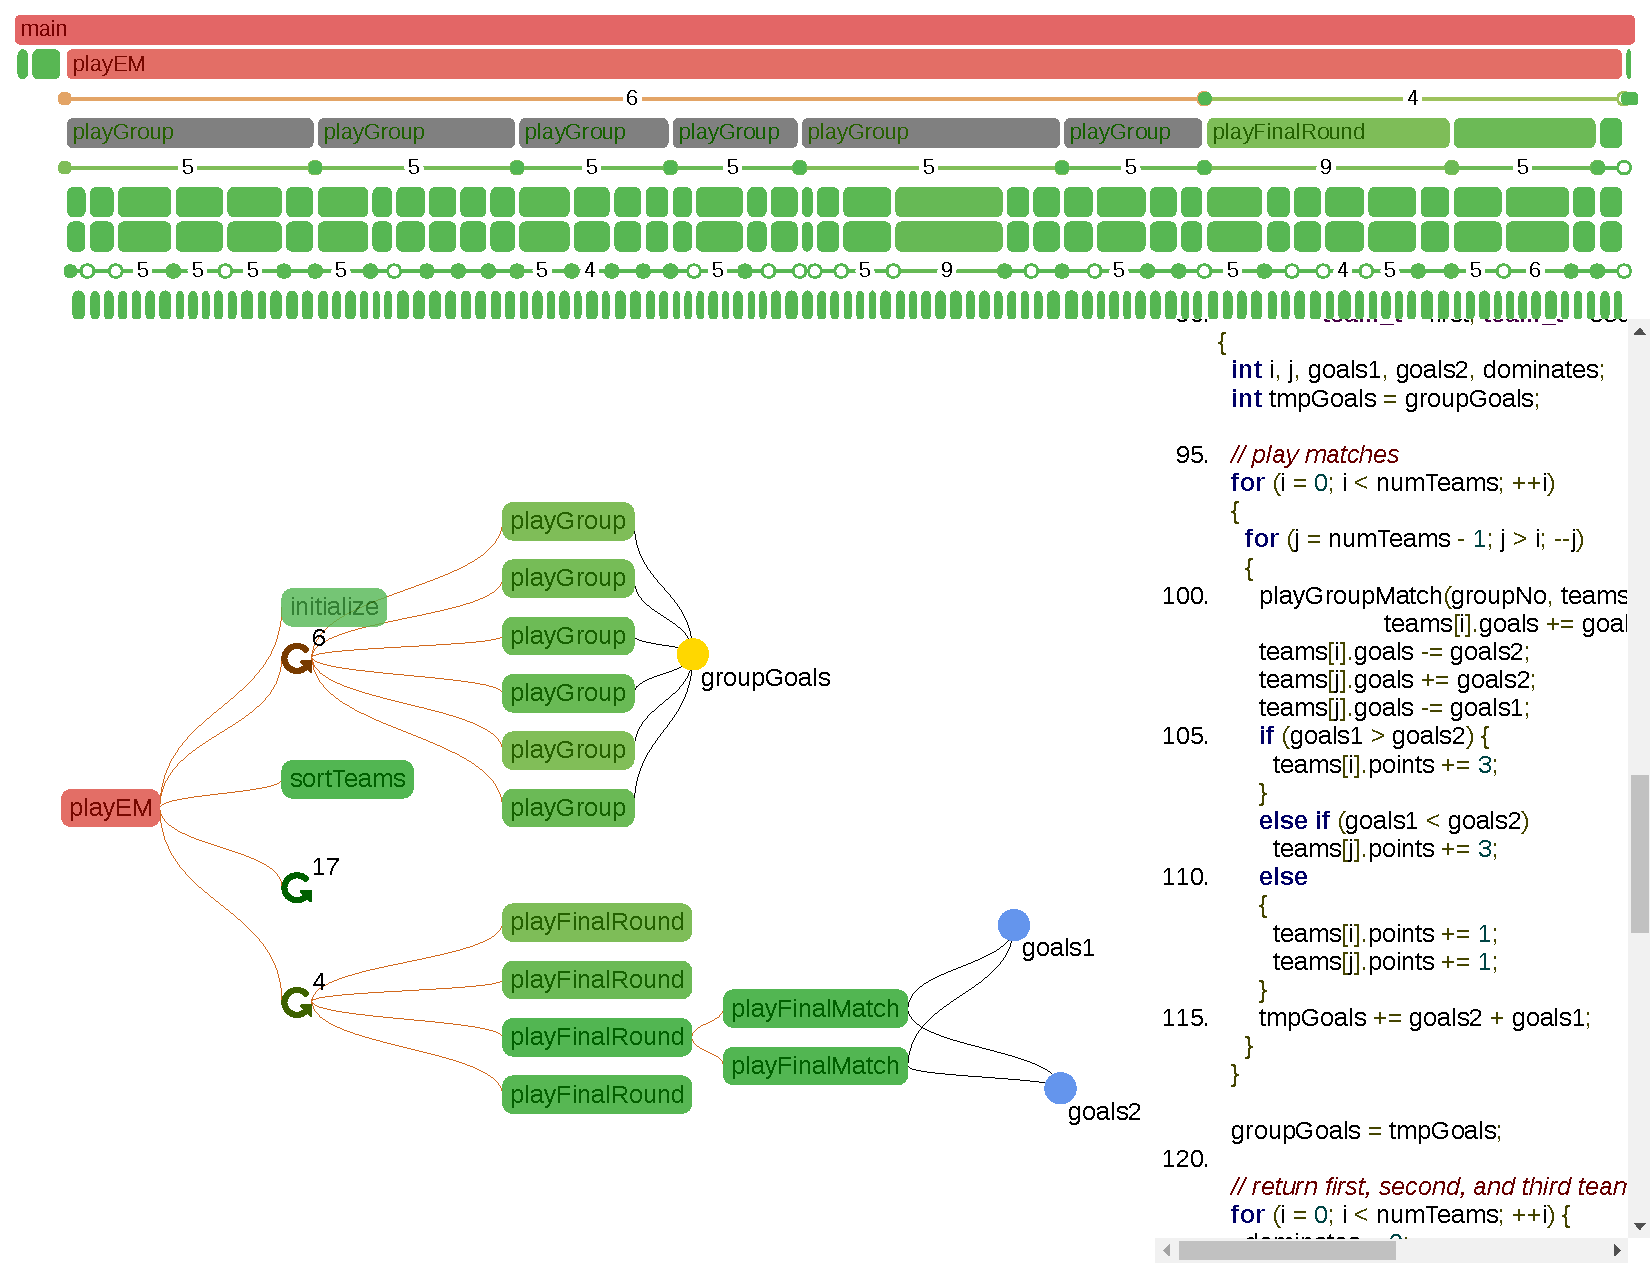
\includegraphics[clip, trim=0.9cm 2.5cm 8.5cm 8.5cm,
width=\linewidth]{img/cct_view}
\caption{The CCT view of Parceive showing function calls (rectangular nodes),
loops, and accessed memory references (circular nodes).}
\label{fig:cct_view}	
\end{figure}

The first node present when the view is created is the call to the
\texttt{main} function. Users can arbitrarily expand and collapse call nodes.
When a function is called multiple times during the same function execution,
the respective call nodes are merged to so-called \textit{call groups}. Call
groups reduce the number of nodes to be displayed but can also be decomposed
into their single call nodes. Navigating through loop executions and loop
iterations is similar to calls and allows the user to see information at any
desired granularity. 

The most important use-case of the CCT view for parallelization is data
dependency analysis. Users are often interested in the existence and the
location of such dependencies between arbitrary regions of their software.
Therefore, optimized queries of the visualization infrastructure are utilized
to detect shared memory accesses across deep call hierarchies. Found
dependencies can then be inspected in a separate source code view. The
described feature allows manageable visualization by dramatically reducing the
amount of shown nodes. There are some additional features that aim for better
scalability and help developers parallelizing their code:

\begin{itemize}
	\item Profiling information (relative execution time) is reflected by node
colors.
	\item Expanding and collapsing nodes can be performed in both
directions to show and hide parent or child nodes.
	\item Seamless zooming, panning, and focusing on single entity nodes for a
better user experience.
	\item Spotting of arbitrary call nodes, which automatically expands the call
tree so that it ends with these nodes and starts with their common ancestor.
\end{itemize}

\subsection{Source View}
The source view shows the source code of the instrumented application, if
available. The usefulness of this view becomes apparent when it is
communicating with the other views presented in this paper. The simplest form
of interaction is focusing, where the source view displays functions, loops,
and memory accesses. Focusing makes it easy to follow the execution of a
program trough the source code. Hovering provides additional information; for
calls it indicates where the call originated, and for memory references where
they were allocated and referenced.